\documentclass{article}
\usepackage[utf8]{inputenc}
\usepackage{amssymb}
\usepackage{graphicx}
\usepackage{amsmath}

\title{CS350 HW5}
\author{Saeah Go}
\date{Due November 5th 2021}

\begin{document}

\maketitle

\section{3.4.1 a, b}
a. Assuming that each tour can be generated in constant time, what will be the efficiency class of the exhaustive-search algorithm outlined in the text for the traveling salesman problem? \\
\indent As there are $n$ cities, in order to calculate the length of the tour, $n$ additions are needed for every hour. \\
\indent \indent $\therefore$ The total number of additions $A(n) = n \; \times$ total number of tours
\indent \indent \indent \indent \indent \indent \indent \indent \indent\indent \indent \indent \indent \indent $= \; n \times \frac{1}{2}(n-1)!$ \\
\indent \indent \indent \indent \indent \indent \indent \indent \indent\indent \indent \indent \indent \indent $= \; \frac{1}{2}n!$ \\
\indent Thus the efficiency class of the given exhaustive search is $\Theta(n!)$ \\ \\
b. If this algorithm is programmed on a computer that makes ten billion additions per second, estimate the maximum number of cities for which the problem can be solved in. \\
\indent Given that a computer can perform 10 billion additions per second which is equal to $10^{10}$ seconds. \\
The total number of additions $ = \frac{1}{2}n!$ \\
And the largest value of $n$ should be determined based on the following inequality: $\frac{1}{2}n!10^{-10} \le t \Longrightarrow n! \le 2 \times 10^{10} \times t$, when $t$ is time in seconds. \\
i. 1 hour \\
\indent Number of seconds in 1 hour is: $60 \times 60$ \\ 
\indent \indent \indent \indent \indent \indent \indent \indent \indent \indent $= 3600$ \\
\indent \indent \indent \indent \indent \indent \indent \indent \indent \indent $= 3.6 \times 10^3$ sec \\
\indent The inequality is $n! \le 2 \times 10^{10}t$ \\
\indent \indent \indent \indent \indent \indent \indent $= \; 2 \times 10^{10} \times 3.6 \times 10^3$ \\
\indent \indent \indent \indent \indent \indent \indent $= \; 7.2 \times 10^{13}$ \\
\indent \indent \indent \indent \indent \indent \indent $\approx 16!$ \indent ($\because 16! = 2.09 \times 10^{12}$) \\
\indent Thus the maximum number of cities for the traveling salesman problem in 1 hour is $16$. \\
ii. 24 hours \\
\indent Number of seconds in 24 hour is: $24 \times 60 \times 60$ \\ 
\indent \indent \indent \indent \indent \indent \indent \indent \indent \indent $\; = 24 \times 3600$ \\
\indent \indent \indent \indent \indent \indent \indent \indent \indent \indent $\; = 86400$ \\
\indent \indent \indent \indent \indent \indent \indent \indent \indent \indent $\; = 8.64 \times 10^4$ sec \\
\indent The inequality is $n! \le 2 \times 10^{10}t$ \\
\indent \indent \indent \indent \indent \indent \indent $= \; 2 \times 10^{10} \times 8.64 \times 10^4$ \\
\indent \indent \indent \indent \indent \indent \indent $= \; 17.28 \times 10^{14}$ \\
\indent \indent \indent \indent \indent \indent \indent $\approx 17!$ \indent ($\because 17! = 3.55 \times 10^{14}$) \\
\indent Thus the maximum number of cities for the traveling salesman problem in 24 hour is $17$. \\
iii. 1 year \\ 
\indent Number of seconds in 1 year is: $365 \times 24 \times 60 \times 60$ \\ 
\indent \indent \indent \indent \indent \indent \indent \indent \indent \indent $\; = 31536000$ \\
\indent \indent \indent \indent \indent \indent \indent \indent \indent \indent $\; = 3.1536 \times 10^7$ sec \\
\indent The inequality is $n! \le 2 \times 10^{10}t$ \\
\indent \indent \indent \indent \indent \indent \indent $= \; 2 \times 10^{10} \times 3.1536 \times 10^7$ \\
\indent \indent \indent \indent \indent \indent \indent $= \; 6.3072 \times 10^{17}$ \\
\indent \indent \indent \indent \indent \indent \indent $\approx 19!$ \indent ($\because 19! = 1.2 \times 10^{17}$) \\
\indent Thus the maximum number of cities for the traveling salesman problem in 1 year is $19$. \\
iv. 1 century \\
\indent Number of seconds in 1 century (100 years) is: $100 \times 365 \times 24 \times 60 \times 60$ \\ 
\indent \indent \indent \indent \indent \indent \indent \indent \indent \indent \indent \indent \indent \indent $\; = 3153600000$ \\
\indent \indent \indent \indent \indent \indent \indent \indent \indent \indent \indent \indent \indent \indent $\; = 3.1536 \times 10^9$ sec \\
\indent The inequality is $n! \le 2 \times 10^{10}t$ \\
\indent \indent \indent \indent \indent \indent \indent $= \; 2 \times 10^{10} \times 3.1536 \times 10^9$ \\
\indent \indent \indent \indent \indent \indent \indent $= \; 6.3072 \times 10^{19}$ \\
\indent \indent \indent \indent \indent \indent \indent $\approx 21!$ \indent ($\because 21! = 5.1 \times 10^{19}$) \\
\indent Thus the maximum number of cities for the traveling salesman problem in 1 century is $21$. 

\section{3.4.2}
Outline an exhaustive-search algorithm for the Hamiltonian circuit problem. \\
1. Assume that the graph contains $n$ vertices. \\
2. Generate a permutation of $n$ vertices such that the permutation starts and \\
\indent ends with the first vertex. \\
3. Then check whether each pair of successive vertices in a current permutation \\
\indent is connected by an edge in the graph. \\
4. If each pair of successive vertices in a current permutation is connected by \\
\indent an edge, then current permutation is the required solution of Hamiltonian \\
\indent circuit. \\
5. Otherwise, generate next permutation to check. \\
6. Do this until all the Hamiltonian circuit is found or all the permutations are \\
\indent tested. 

\section{3.5.1 a,b}
Consider the following graph.
\begin{center}
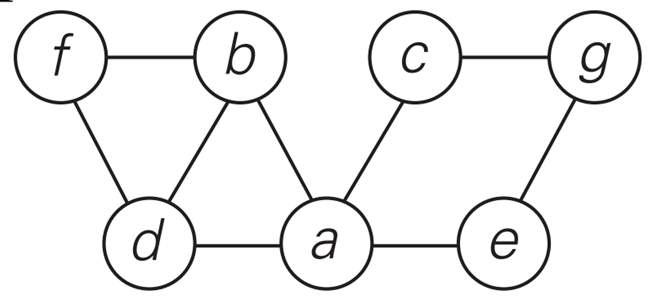
\includegraphics[scale = 0.5]{graph.png} \\
\end{center}
a. Write down the adjacency matrix and adjacency lists specifying this graph.
(Assume that the matrix rows and columns and vertices in the adjacency
lists follow in the alphabetical order of the vertex labels.) \\
\indent Adjacency Matrix Representation: In a graph if there is a direct edge between vertex \textit{a} and vertex \textit{b} then value of \textit{a} to \textit{b} in adjacency matrix is 1. Otherwise, we take 0 in the adjacency matrix.
\begin{center}
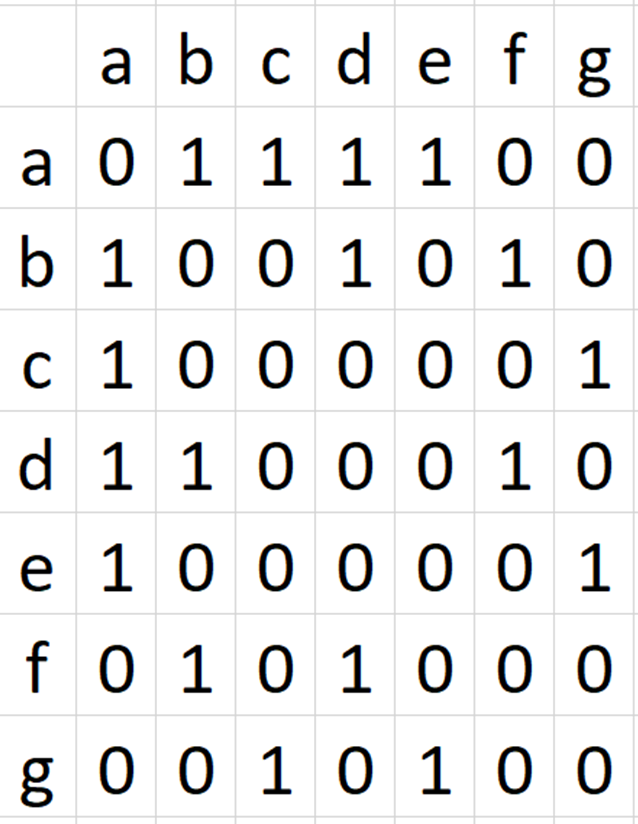
\includegraphics[scale = 0.3]{adjacency matrix.png} \\
\end{center} 
\indent \indent The adjacency List Representation is: \\
\indent \indent \indent a $\; \longrightarrow \; $ b $\; \longrightarrow \;$ c $\; \longrightarrow \;$ d $\; \longrightarrow \;$ e \\
\indent \indent \indent b $\; \longrightarrow \; $ a $\; \longrightarrow \;$ d $\; \longrightarrow \;$ f \\
\indent \indent \indent c $\; \longrightarrow \; $ a $\; \longrightarrow \;$ g \\
\indent \indent \indent d $\; \longrightarrow \; $ a $\; \longrightarrow \;$ b $\; \longrightarrow \;$ f \\
\indent \indent \indent e $\; \longrightarrow \; $ a $\; \longrightarrow \;$ g \\
\indent \indent \indent f $\; \longrightarrow \; $ b $\; \longrightarrow \;$ d \\
\indent \indent \indent g $\; \longrightarrow \; $ c $\; \longrightarrow \;$ e 

b. Starting at vertex a and resolving ties by the vertex alphabetical order, traverse the graph by depth-first search and construct the corresponding depth-first search tree. Give the order in which the vertices were reached for the first time (pushed onto the traversal stack) and the order in which the vertices became dead ends (popped off the stack). \\
Step 1: We have the starting vertex `\textit{a}', so first push it in the stack. \\
\indent \indent \indent Push order: a \\
Step 2: Adjacent nodes of `\textit{a}' are \textit{`b', `c', `e' and `d'}. And we need to follow alphabetical order, so push `\textit{b}' in stack. \\
\indent \indent \indent Push order: a, b \\
Step 3: Adjacent nodes of `\textit{b}' are \textit{`a', `f' and `d'}. Since we have already traversed `\textit{a}', ignore `\textit{a}'. As we have to follow alphabetical order, push `\textit{d}' in stack. \\
\indent \indent \indent Push order: a, b, d \\
Step 4: Adjacent nodes of `\textit{d}' are \textit{`a', `b' and `f'}. But since we have already traversed `\textit{a}' and `\textit{b}', ignore them and push `\textit{f}' in stack. \\
\indent \indent \indent Push order: a, b, d, f \\
Step 5: We reached the dead end, so back tracking and popping `\textit{f}' from the stack. Then,
\indent \indent \indent Push order: a, b, d, f \\
\indent \indent \indent Pop order: f \\
Step 6: After backtracking, we reached `\textit{d}' but from `\textit{d}' we have visited all the vertex. So pop `\textit{d}' from the stack. \\
\indent \indent \indent Push order: a, b, d, f \\
\indent \indent \indent Pop order: f, d \\
Step 7: Again, after backtracking, we reached `\textit{b}' but from `\textit{b}' we have visited all the vertex. So pop `\textit{b}' from the stack. 
\indent \indent \indent Push order: a, b, d, f \\
\indent \indent \indent Pop order: f, d, b \\
Step 8: Now we reached `\textit{a}', and from `\textit{a}' we still have not visited all the vertex. The adjacent nodes of `\textit{a}' are \textit{`b', `c', `e' and `d'}. We already visited \textit{`b' and `d'} so we don't have to worry about those. We have to follow alphabetical order, so push \textit{`c'} in stack. \\
\indent \indent \indent Push order: a, b, d, f, c \\
\indent \indent \indent Pop order: f, d, b \\
Step 9: The adjacent of \textit{`c'} are \textit{`a' and `g'}. But we already visited \textit{`a'} so push \textit{`g'} in stack. \\
\indent \indent \indent Push order: a, b, d, f, c, g \\
\indent \indent \indent Pop order: f, d, b \\
Step 10: The adjacent nodes of \textit{`g'} are \textit{`c' and `e'}. But we already visited \textit{`c'} so push \textit{`e'} in stack. \\
\indent \indent \indent Push order: a, b, d, f, c, g, e \\
\indent \indent \indent Pop order: f, d, b \\
Step 11: We reached the dead end, so backtracking and popping \textit{`e'} from the stack. \\
\indent \indent \indent Push order: a, b, d, f, c, g, e \\
\indent \indent \indent Pop order: f, d, b, e \\
Step 12: Now we have visited all the vertices, so simply backtrack and pop the elements from the stack in reverse order. So final push order and pop order are:
\indent \indent \indent Push order: a, b, d, f, c, g, e \\
\indent \indent \indent Pop order: f, d, b, e, g, c, a \\ \\ 
\textbf{Conclusion:} \\
The order in which vertices were reached for the first time (pushed onto the traversal stack) is a, b, d, f, c, g, e.  \\
The order in which the vertices became dead ends (popped off the stack) is f, d, b, e, g, c, a.

\section{3.5.2}
If we define sparse graphs as graphs for which $|E| \; \epsilon \; O(|V|)$, which implementation of DFS will have a better time efficiency for such graphs, the one that uses the adjacency matrix or the one that uses the adjacency lists? \\
Time efficiency of DFS for Adjacency Matrix $= \Theta(\lvert V\rvert^2)$ \\
Time efficiency of DFS for Adjacency Lists $= \Theta(\lvert V\rvert + \lvert E \rvert)$ \\
Sparse graphs are defined as graphs for which $\lvert E\rvert \; \epsilon \; \Theta(\lvert V\rvert)$. Then, \\
Time efficiency of DFS for Sparse graphs using Adjacency Matrix $= \Theta(\lvert V\rvert^2)$ \\
Time efficiency of DFS for Sparse graphs using Adjacency Lists $= \Theta(\lvert V\rvert + \lvert E \rvert) = \Theta(\lvert V \rvert) \indent (\because \lvert E\rvert \; \epsilon \; \Theta(\lvert V\rvert)$ \\
We know that $\Theta(\lvert V\rvert)$ is more efficient than $\Theta(\lvert V\rvert^2)$ \\
In other words, for sparse graphs, adjacency list implementation of DFS is more efficient.

\section{3.5.6 a,b}
a. Explain how one can check a graph’s acyclicity by using breadth-first search. \\
\indent We know that a graph has a cycle if its BFS forest has a cross edge. We can check it by increasing a counter when we visit a node in BFS. If the counter becomes larger than N * N before the traversal is complete, then there is a cycle. If the traversal is complete and the counter is not larger than N * N, then there is no cycle. \\
b. Does either of the two traversals—DFS or BFS—always find a cycle faster than the other? If you answer yes, indicate which of them is better and explain why it is the case; if you answer no, give two examples supporting your answer. \\
\indent DFS always finds a cycle faster than BFS. Depth first search is more memory efficient than breadth first search as we can backtrack sooner. It is also easier to implement if we use the call stack but this relies on the longest path not overflowing the stack. Thus DFS finds a cycle faster than BFS.


\section{3.5.7}
Explain how one can identify connected components of a graph by using \\
a. a depth-first search. \\
\indent 1. Create a set of vertices that are not visited in the graph. \\
\indent 2. Then, create an empty set which can be used to keep track of nodes which have been already visited. \\
\indent 3. From the set of unvisited vertex, choose a vertex and start exploring the graph. \\
\indent 4. Begin with depth-first traversal from the node. For this, remove the nodes which are already visited from the set of unvisited nodes. Now, add those removed nodes in the set of visited nodes. \\
\indent 5. After this, when the depth first traversal is completed, show the nodes that are in the visited set. These nodes will represent the connect components. \\
\indent 6. Now, empty the nodes in the visited set. \\
\indent 7. If the unvisited set is still not empty then, repeat from step 3 again. \\
\indent 8. Otherwise, if the unvisited set is empty, then there are no more connected components left. \\ \\
b. a breadth-first search. \\
\indent 1. Create a set of vertices that are not visited in the graph. \\
\indent 2. Then, create an empty set which can be used to keep track of nodes which have been already visited. \\
\indent 3. From the set of unvisited vertex, choose a vertex and start exploring the graph. \\
\indent \indent Also. add that vertex to a queue. \\
\indent 4. Insert the selected vertex into the queue. \\
\indent 5. Now, remove a vertex from the queue and insert all the vertices that are connected to this inserted in the queue. \\
\indent 6. Add the vertex that is removed to the visited set. \\
\indent 7. If the queue is not empty then again move to step 5 and start from that step 5 again. \\
\indent 8. Otherwise, show the components of the visited set. These nodes that are being displayed will represent the connected components. \\
\indent 9.Now, clear the content of the visited set. \\
\indent 10. If the unvisited set is still not empty then, repeat from step 3 again. \\
\indent 11. Otherwise, if the unvisited set is empty, then there are no more connected components left.

\end{document}
